\documentclass{article}
\title{Computer Workshop \\ Final Assignment}
\author{Ali Mozdianfard}
\date{January 2024}

\usepackage{graphicx}

\begin{document}
	\maketitle
	\newpage
	
	\tableofcontents
	\newpage
	
	\section{Git \& GitHub}
	Here is every step of the process of creating the repository of this assignment
	and setting up the GitHub Actions for compiling \LaTeX.
	
	\begin{figure}[h]
		\centering
		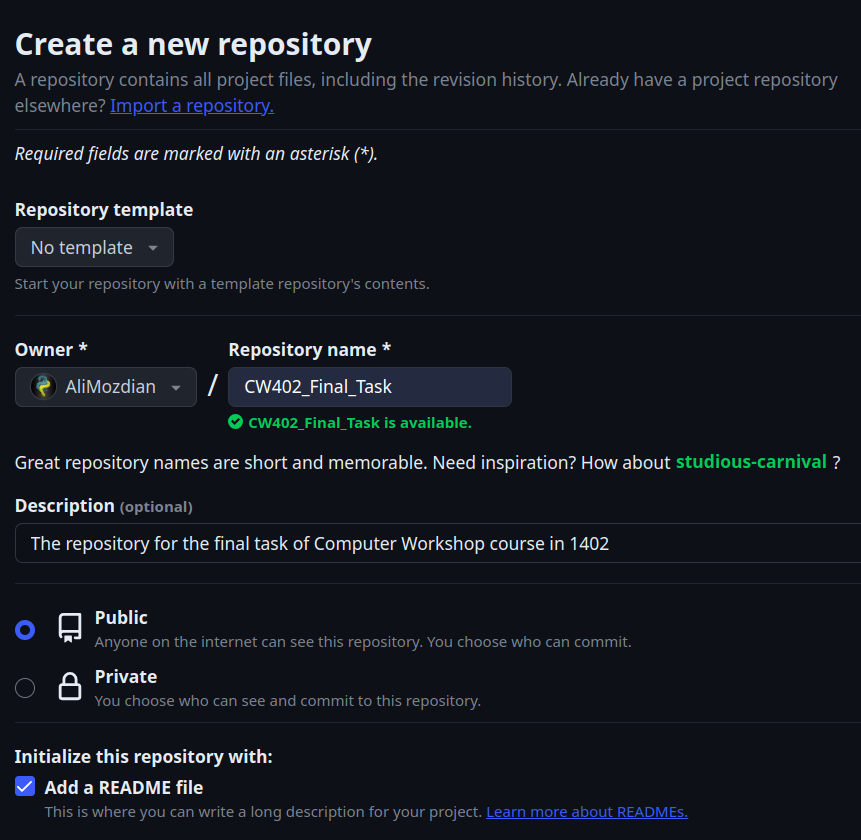
\includegraphics[width=\textwidth]{images/ss0.png}
		\caption{Creating the repository in GitHub}
	\end{figure}
	
	\begin{figure}[h]
		\centering
		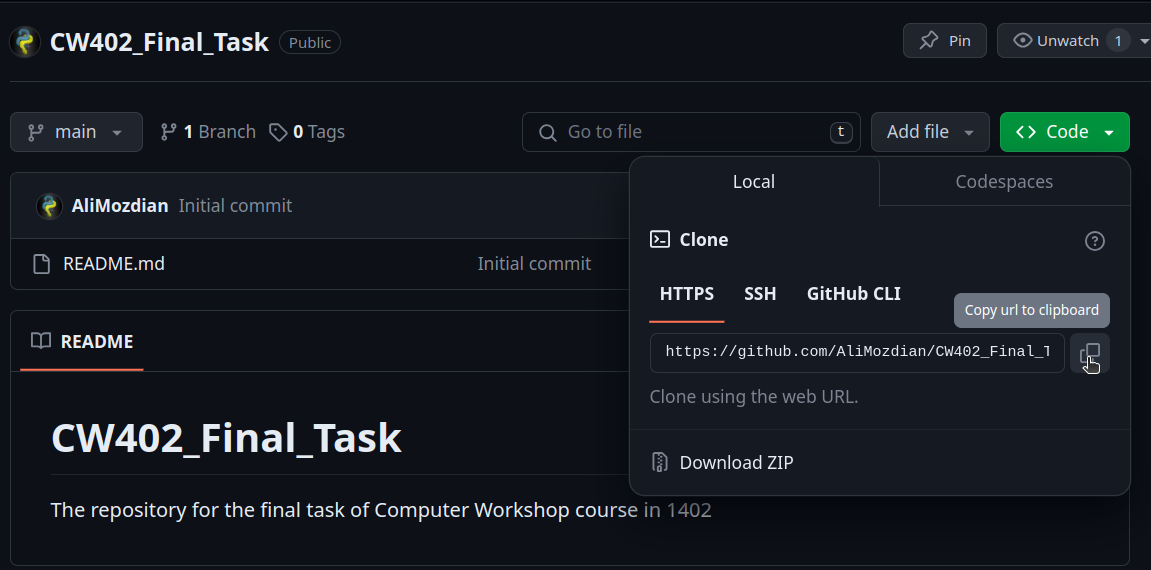
\includegraphics[width=\textwidth]{images/ss1.png}
		\caption{Copying the link of HTTPS link for cloning the repository into my local machine}
	\end{figure}
	
	\begin{figure}[h]
		\centering
		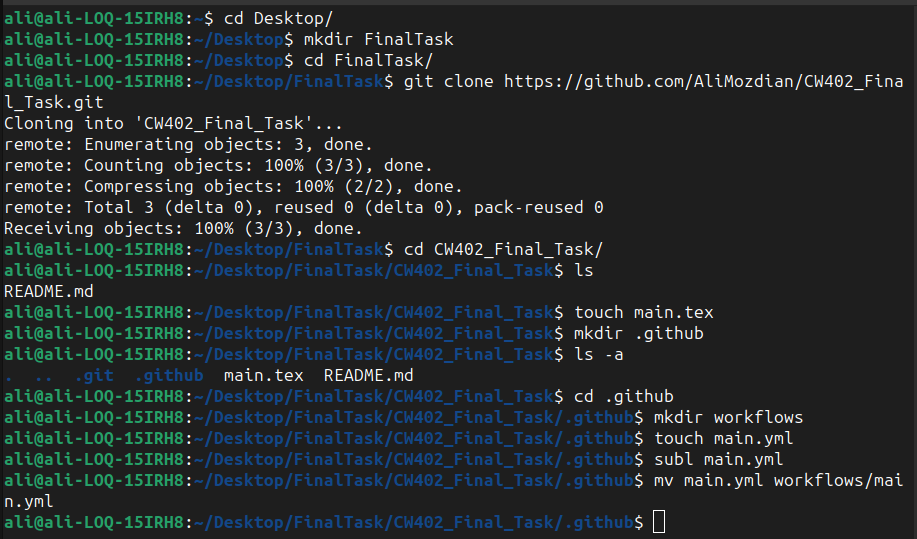
\includegraphics[width=\textwidth]{images/ss2.png}
		\caption{From now on we will be doing the needed setup for GitHub Actions. \\ Creating the needed files for the project.}
	\end{figure}
	
	\begin{figure}[h]
		\centering
		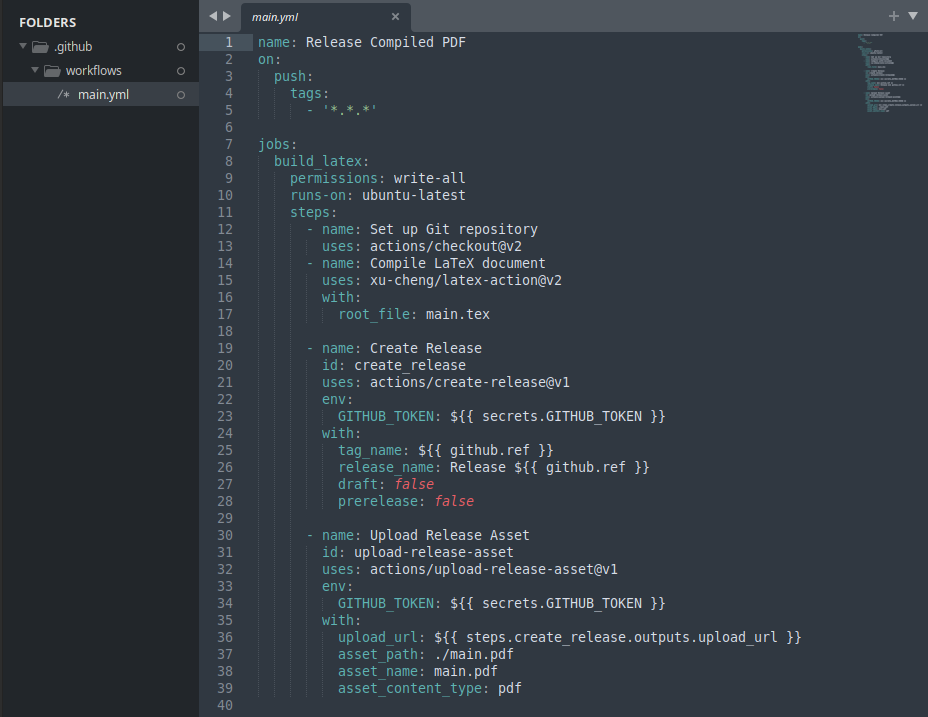
\includegraphics[width=\textwidth]{images/ss3.png}
		\caption{Writing in main.yml to set GitHub Actions (.github/workflows/main.yml)}
	\end{figure}
	
	\begin{figure}[h]
		\centering
		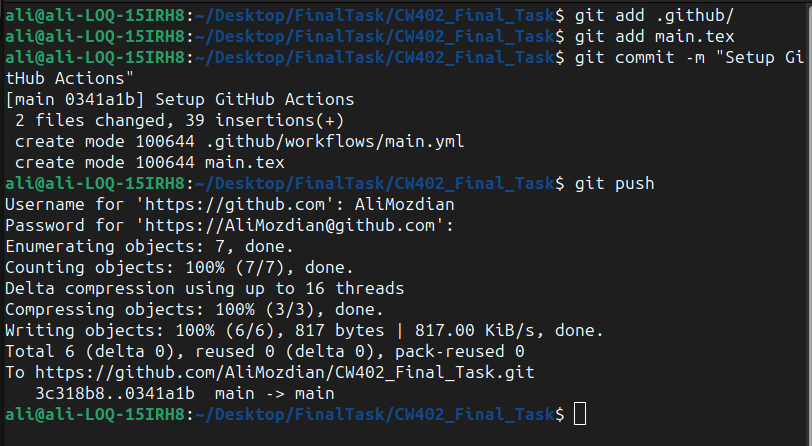
\includegraphics[width=\textwidth]{images/ss4.png}
		\caption{add, commit and push, then we are ready to start the project, but tags!}
	\end{figure}
	
	\begin{figure}[h]
		\centering
		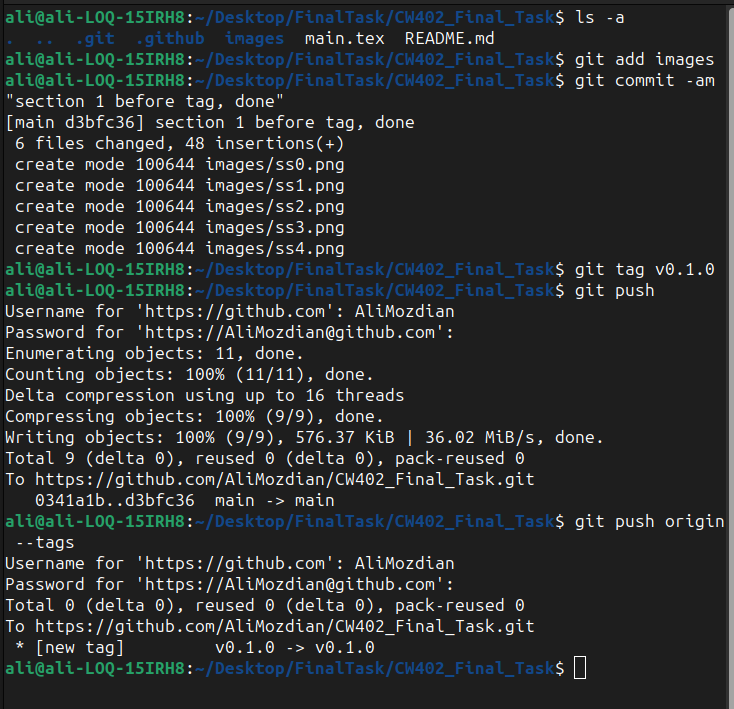
\includegraphics[width=\textwidth]{images/ss5.png}
		\caption{Adding and commiting the images, also making a tag for this commit. \\ then pushing the repo and its tags (via two commands)}
	\end{figure}
	
	\begin{figure}[h]
		\centering
		
\includegraphics[width=\textwidth]{images/ss6.png}
		\caption{As you can see the tags now are in GitHub as well}
	\end{figure}
	
	\begin{figure}[h]
		\centering
		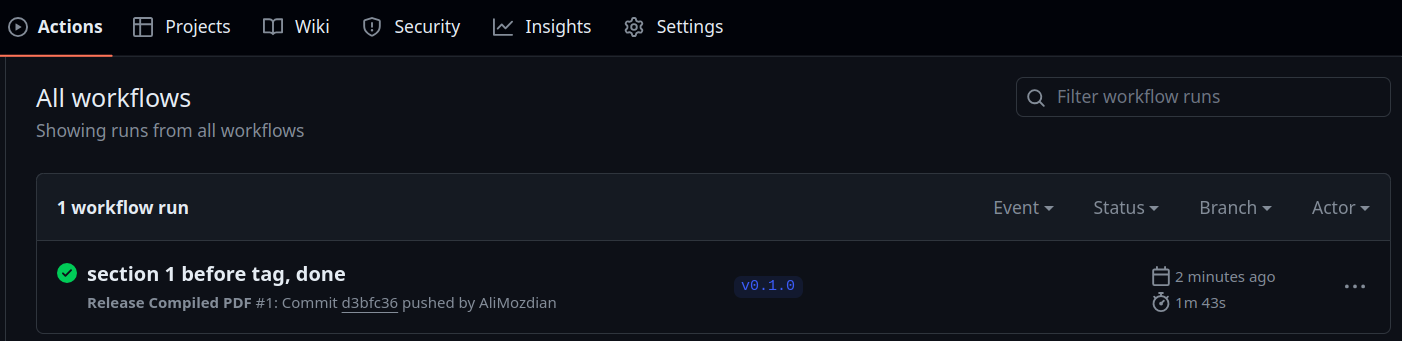
\includegraphics[width=\textwidth]{images/ss7.png}
		\caption{And becuase of the format of the tag, GitHub Actions complied it without a problem}
	\end{figure}
	
	So just repeat this cycle:
	\begin{enumerate}
		\item make changes
		\item git add
		\item git commit
		\item git tag
		\item git push
		\item git push tags
		\item GitHub Actions compiles the main.tex automatically
	\end{enumerate}

\end{document}
